% Methods: here you generally use the passive voice in the simple past.
\section{Methodology} \label{section:methodology}


% All assets to build the environment have been available through the free game asset website www.kenney.nl

\subsection{The game} \label{subsection:game}
The objective of the game is to survive five days in the wilderness.
The wilderness has resources in the form of mushrooms.
% and threats in the form of snakes.
A world clock is displayed, in order to know how far into the simulation we are.
Furthermore, in the top left corner of the screen, information about the simulation is displayed.

\subsection{The environment} \label{subsection:environment}
The environment consists of a grid, in which cuboids are drawn in the isometric projection, in order to achieve a faux 3D environment, or more appropriately, 2.5D environment.
These individual cuboids are referred to as the grass tiles.
The grass tiles were then used to draw objects upon then.
These objects include trees and rocks.
The majority of the environment consists of trees, as Perlin noise was used to create forests in the game environment \cite[Chapter~4]{shaker2016procedural,perlin1985image}.
Using a probability of one per cent each, rocks and singular trees are placed as well.
Additionally, these objects were assigned a collision variable, such as the boundaries of the environment.
This variable was used to detect obstacle collisions between sprites and the environment and to keep said sprites within the boundaries of the environment.    
Lastly, a base location, depicted by a large red flag, is spawned together with the agents.


\subsection{Camera} \label{subsection:camera}
% find a more fitting word than "handle"
A scrolling camera was implemented to handle maps that are larger than the screen. 
Based on the position of the mouse on the screen, the camera can scroll in any of the four directions.
The offset created by scrolling was added dynamically to the sprites in the environment, in order to correct their position.

% resources, kenney.nl
\subsection{Physics} \label{subsection:physics}
The instances in the environment are represented as vectors.
In order to move said instances, vector calculus is applied.
A standard rotation matrix (\ref{equations:vector_rotation}) is used to rotate the matrix by a random $\theta$.

\begin{equation}[H]
    R(\theta)=\left[\begin{array}{cc}
    \cos \theta & -\sin \theta \\
    \sin \theta & \cos \theta
    \end{array}\right]
    \label{equations:vector_rotation}
\end{equation}

The vectors are normalized (\ref{equations:normalized_vector}) to become $\mathbf {\hat {u}}$, 
furthermore euclidean norm (\ref{equations:euclidean_norm}) is used for the norm $|\mathbf {u} |$.

\begin{equation}[H]
    \mathbf {\hat {u}} ={\frac {\mathbf {u} }{|\mathbf {u} |}}
    \label{equations:normalized_vector}
\end{equation}
\begin{equation}[H]
    \left\|{\mathbf {x}}\right\|_{2}:={\sqrt {x_{1}^{2}+\cdots +x_{n}^{2}}}
    \label{equations:euclidean_norm}
\end{equation}

\subsection{Agent} \label{subsection:agent}
% see for original: buckland p. 86

An agent is depicted by a sprite.
\textcolor{blue}{---
Each agent has its own health and energy levels, which get depleted during the simulation.
Upon hovering with the mouse above an agent, health and energy bars are displayed.
Accordingly, energy levels can be replenished, where health cannot.
Agents also have a predefined maximum and minimum speed and mass.
---}


Each agent in the environment is controlled by a Finite State Machine.
The behaviours are triggered in these FSM by thresholds and boolean expressions.
The FSM of the agents is depicted below in Figure \ref{fig:agent_FSM}.

Regarding the movement of the agents, two driving forces can be identified.
These are \textbf{action selection} and \textbf{steering}.
The former determines the immediate goal to be achieved by the agent, as can be seen in the FSM.
Ultimately, to achieve the goal set by action selection, steering is needed.
The mechanism is responsible for calculating the desired trajectories required to carry out the selected action.
For steering to be applied, a steering force is necessary.
This force describes the direction and velocity of the desired displacement.

\usetikzlibrary{automata,positioning,arrows}
\tikzset{
    ->, 
>=stealth, 
node distance=5cm,
every state/.style={thick, fill=gray!10},
initial text=$ $,}

\begin{figure}[H]
    \centering
    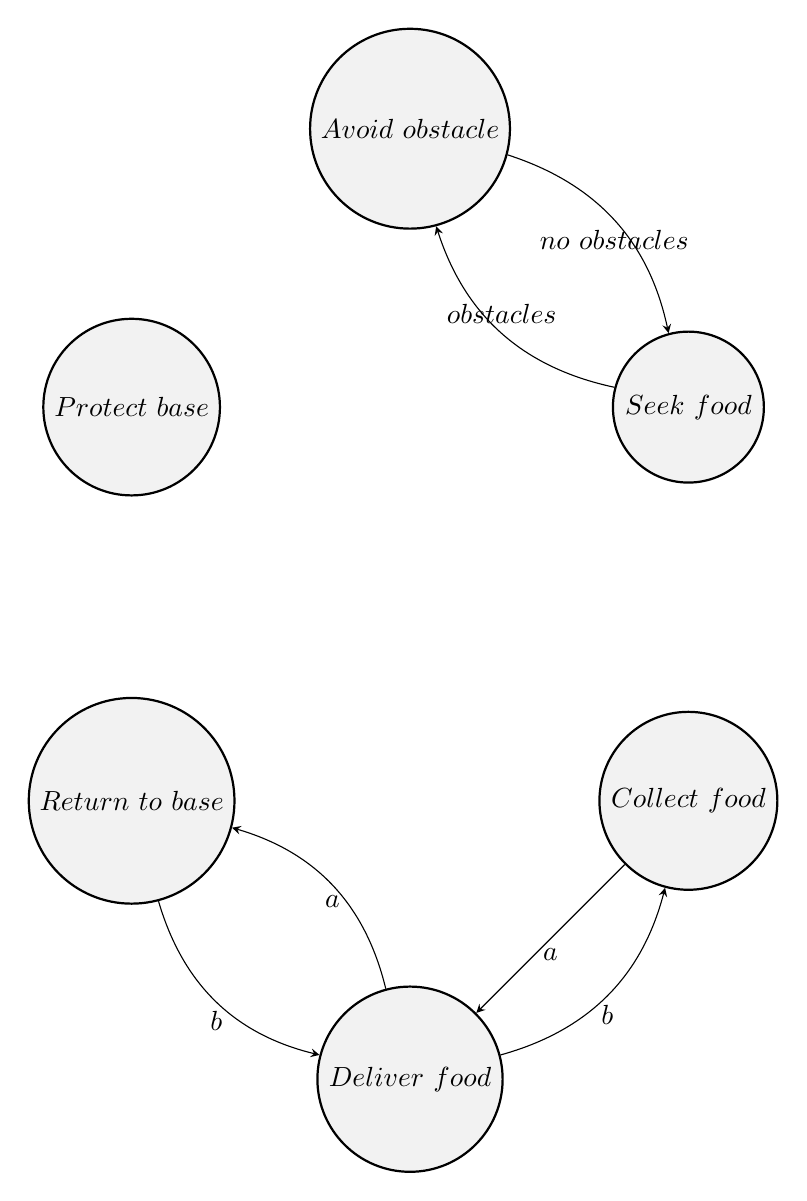
\begin{tikzpicture}
        \node[state] (1) {$Avoid\ obstacle$};
        \node[state, below left of=1] (2) {$Protect\ base$};
        \node[state, below right of=1] (3) {$Seek\ food$};
        \node[state, below of=3] (4) {$Collect\ food$};
        \node[state, below left of=4] (5) {$Deliver\ food$};
        \node[state, below of=2] (9) {$Return\ to\ base$};
        % \node[state, below  left of=1] (6) {$Flee\ enemy$};
        % \node[state, below  of=6] (7) {$Towards\ enemy$};
        % \node[state, below  of=7] (8) {$Attack\ enemy$};
        \draw
        (1) edge[below, bend left] node{$no\ obstacles$} (3)
        (3) edge[above, bend left] node{$obstacles$} (1)
        % (1) edge[below, bend right] node{$no\ obstacles$} (6)
        % (6) edge[above, bend right] node{$obstacles$} (1)
    
        (4) edge[below] node{$a$} (5)
        (5) edge[below, bend right] node{$b$} (4)
    
        (5) edge[below, bend right] node{$a$} (9)
        (9) edge[below, bend right] node{$b$} (5)
    
        ;
    \end{tikzpicture}
    \caption{Agent FSM}
    \label{fig:agent_FSM}
\end{figure}




\subsection{Behaviours} \label{subsection:behaviours}
Each agent has the ability to carry out a number of behaviours. 
The priority for carrying out the behaviours depend on the environment.
% When the environment is devoid of resources and threats, the agents wander in the perimeter of the home base.
If they encounter an obstacle, the aim is to avoid collision.
Failing to do so, they take damage until they get away from the obstacle.
When food is available, the agents start foraging, see Algorithm \ref{algorithm:seek}. 
A group of agents walks towards the food item, and collects it.
The agent that collected the mushroom, switches from foraging to delivering.
With a delivering task, the agent is entrusted to bring the mushroom back to the base.
When enough food is available at the base, the agents can return and stay at the base to replenish their health.
% Lastly, when there are threats in the environment, the agents need to be careful.
% If a snake comes close, the agent has to determine whether to flee \ref{algorithm:flee}, or to attack.
% The choice depends on availability of companions in the vicinity.
% Without other agents nearby, the agent flees, otherwise it attacks the enemy.
In all of the scenarios, the movements of the agents are affected by forces derived from their neighbors.
These forces include, alignment forces, cohesion forces and separation forces.


% https://en.wikibooks.org/wiki/LaTeX/Algorithms#Typesetting_using_the_algorithmic_package
% see buckland page 91 - 125
\subsubsection*{Seek}
The \textbf{seek} steering behaviour returns a force that directs an agent toward a target position.
% This behaviour is activated when the agent decides to attack the enemy.
% In our engine, this is determined by having the required number of neighbours in the vicinity.

\begin{algorithm}[H]
    \caption{Seek steering behavior}
    \begin{algorithmic}[1]
        \State desired\_velocity = target\_pos - agent\_pos
        \State desired\_velocity = normalize(desired\_velocity)
        \State \Return desired\_velocity
    \end{algorithmic}
    \label{algorithm:seek}
\end{algorithm}





\subsubsection*{Deliver}
The \textbf{deliver} steering behaviour is triggered when an agent collects a mushroom.
A force is returned that steers the agent towards the home base.

\begin{algorithm}[H]
    \caption{Food delivering steering behavior}
    \begin{algorithmic}[1]
        \State desired\_velocity = agent\_pos - target\_pos
        \State \Return desired\_velocity
    \end{algorithmic}
    \label{algorithm:deliver}
\end{algorithm}



\subsubsection*{Protect}
The \textbf{protect} steering behaviour is activated when the collective health of the swarm reaches a threshold.
Agents that are within the vicinity of the home base, stay inside the perimeter, 
while those that have wandered outside the perimeter return a force that steers them towards the base.

\begin{algorithm}[H]
    \caption{Base protection steering behavior}
    \begin{algorithmic}[1]
        \State desired\_velocity = agent\_pos - target\_pos
        \State \Return desired\_velocity
    \end{algorithmic}
    \label{algorithm:protect}
\end{algorithm}



% buckland p.99
\subsubsection*{Obstacle avoidance}
\textbf{Obstacle avoidance} aims to steer agents away from obstacles that are in their path.
The identification of two tiles are necessary for this behaviour; 
namely the tile on which the obstacle is placed and the tile on which the agent currently is located.
If the trajectory of the agent is towards the obstacle tile, and the distance is less than one tile;
then the obstacle avoidance behaviour is triggered.


\begin{algorithm}[H]
    \caption{Tile based obstacle avoidance steering behavior}
    \begin{algorithmic}[1]
        \State desired\_velocity = agent\_pos - target\_pos
        \State \Return desired\_velocity
    \end{algorithmic}
    \label{algorithm:avoid}
\end{algorithm}



\subsubsection*{Wander}
The \textbf{wander} steering behaviour returns a force that directs an agent towards a random location.
\begin{algorithm}[H]
    \caption{Wandering steering behavior}
    \begin{algorithmic}[1]
        \State desired\_velocity = agent\_pos - target\_pos
        \State \Return desired\_velocity
    \end{algorithmic}
    \label{algorithm:wander}
\end{algorithm}





% https://github.com/mdodsworth/pyglet-boids
\subsubsection*{Alignment}
\begin{algorithm}[H]
    \caption{Alignment collective steering behavior}
    \begin{algorithmic}[1]
        \State desired\_velocity = agent\_pos - target\_pos
        \State \Return desired\_velocity
    \end{algorithmic}
    \label{algorithm:alignment}
\end{algorithm}


In \textbf{alignment}, the velocity of an agent is manipulated to match that of its neighbours.

\begin{algorithm}[H]
    \caption{Alignment collective steering behavior}
    \begin{algorithmic}[1]
        \State desired\_velocity = agent\_pos - target\_pos
        \State \Return desired\_velocity
    \end{algorithmic}
    \label{algorithm:alignment}
\end{algorithm}



\subsubsection*{Cohesion}
\begin{algorithm}[H]
    \caption{Cohesion collective steering behavior}
    \begin{algorithmic}[1]
        \State desired\_velocity = agent\_pos - target\_pos
        \State \Return desired\_velocity
    \end{algorithmic}
    \label{algorithm:cohesion}
\end{algorithm}



The \textbf{cohesion} collective behaviour steers each agent to the geometric center of all nearby agents.

\begin{algorithm}[H]
    \caption{Cohesion collective steering behavior}
    \begin{algorithmic}[1]
        \State desired\_velocity = agent\_pos - target\_pos
        \State \Return desired\_velocity
    \end{algorithmic}
    \label{algorithm:cohesion}
\end{algorithm}



\subsubsection*{Separation}
\textbf{Separation} attemps to steer agents away from others, in order to prevent them crowding each other.
The algorithm iterates over all the perceived neighbours of the agent.
The vector to each neighbour is then normalized and divided by the distance to the neighbour.
This vector is then added to the steering force. 
\begin{algorithm}[H]
    \caption{Separation collective steering behavior}
    \begin{algorithmic}[1]
        \State desired\_velocity = agent\_pos - target\_pos
        \State steering\_force += normalized(distance\_to\_neighbour) / num\_neighbours
        \State \Return steering\_force
    \end{algorithmic}
    \label{algorithm:separation}
\end{algorithm}



\begin{algorithm}[H]
    \caption{Separation collective steering behavior}
    \begin{algorithmic}[1]
        \State desired\_velocity = agent\_pos - target\_pos
        \State steering\_force += normalized(distance\_to\_neighbour) / num\_neighbours
        \State \Return steering\_force
    \end{algorithmic}
    \label{algorithm:separation}
\end{algorithm}



\subsection{Swarm} \label{subsection:swarm}
The agents were grouped into a sprite group, called the swarm. 
A high level representation of the swarm is depicted in Figure \ref{fig:swarm}.
When an agent in the swarm reaches a health level of zero, it dies and is removed from the swarm.

\tikzset{
    ->, 
>=stealth, 
node distance=5cm,
every state/.style={thick, fill=gray!10},
initial text=$ $,}

\begin{figure}[H]
    \centering
    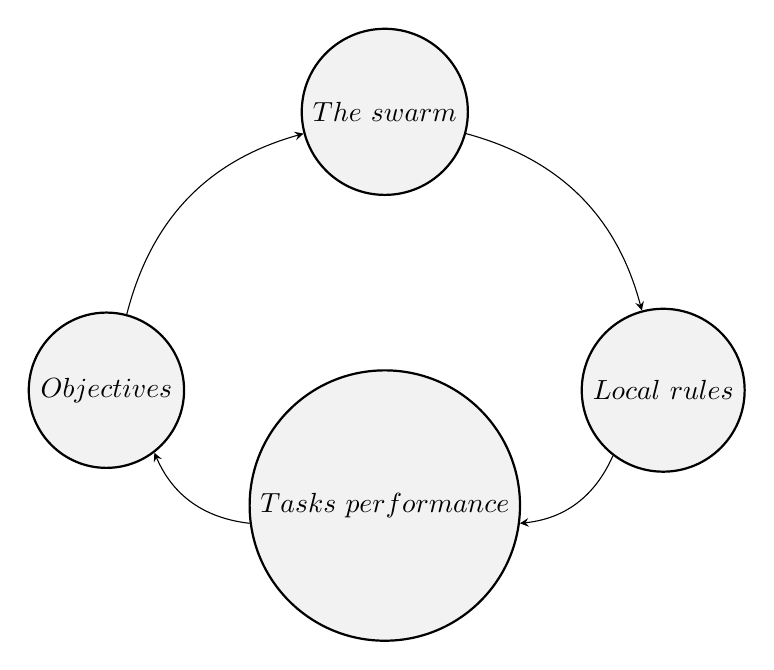
\begin{tikzpicture}
        \node[state] (1) {$The\ swarm$};
        \node[state, below right of=1] (2) {$Local \ rules$};
        \node[state, below  of=1] (3) {$Tasks\ performance$};
        \node[state, below left of=1] (4) {$Objectives$};
        \draw
        (1) edge[below, bend left] (2)
        (2) edge[below, bend left] (3)
        (3) edge[below, bend left] (4)
        (4) edge[below, bend left] (1)
    
        ;
    \end{tikzpicture}
    \caption{Swarm representation}
    \label{fig:swarm}
\end{figure}

% adapted from: Swarm Intelligence in Data Mining




\subsection{Food} \label{subsection:food}
The available food in the wilderness are mushrooms.
\textcolor{blue}{---
Consuming these mushrooms replenishes the energy and health of the agents. 
---}



